\documentclass[10pt]{article}
\usepackage{cs535}
\usepackage{amsmath,amssymb,amsthm,mathtools}
\usepackage{algorithm}
\usepackage[noend]{algpseudocode}
\usepackage{booktabs,array,graphicx,microtype,url}
\usepackage[hidelinks]{hyperref}
\usepackage[capitalise,nameinlink]{cleveref}

% ---------- theorem environments (shared counter) ----------
\newtheoremstyle{tplain}{2pt}{2pt}{\itshape}{}{\bfseries}{.}{.5em}{}
\newtheoremstyle{tdef}{2pt}{2pt}{\normalfont}{}{\bfseries}{.}{.5em}{}
\newtheoremstyle{trem}{2pt}{2pt}{\normalfont}{}{\itshape}{.}{.5em}{}
\theoremstyle{tplain}
\newtheorem{theorem}{Theorem}
\newtheorem{lemma}[theorem]{Lemma}
\newtheorem{proposition}[theorem]{Proposition}
\newtheorem{fact}[theorem]{Fact}
\theoremstyle{tdef}
\newtheorem{assumption}{Assumption}
\renewcommand{\theassumption}{A\arabic{assumption}}
\theoremstyle{trem}
\newtheorem{remark}[theorem]{Remark}
\crefname{assumption}{Assumption}{Assumptions}
\crefname{fact}{Fact}{Facts}
\crefname{algorithm}{Algorithm}{Algorithms}

% ---------- macros ----------
\newcommand{\R}{\mathbb{R}}
\newcommand{\E}{\mathbb{E}}
\newcommand{\Hbar}{\bar H}
\newcommand{\epss}{\varepsilon_s}
\newcommand{\epsv}{\varepsilon_v}
\newcommand{\etaNL}{\eta_{\mathrm{NL}}}
\newcommand{\Qhat}{\hat Q}
\newcommand{\Qstar}{Q^\star}
\newcommand{\Vstar}{V^\star}
\newcommand{\Abar}{\bar A}
\newcommand{\qhat}{\hat q}
\newcommand{\cS}{\mathcal S}
\DeclareMathOperator{\val}{val}
\DeclareMathOperator{\expl}{expl}
\DeclareMathOperator{\TV}{TV}
\DeclareMathOperator{\Reg}{Reg}
\DeclareMathOperator{\KL}{KL}
\DeclareMathOperator{\clip}{clip}
\DeclareMathOperator{\gap}{gap}

\title{No-Regret Learning and Bayesian Opponent Memory\\in Pok\'emon Random Battles}
\author{[Names]\\ \normalfont CS535 Final Project}

\begin{document}
\maketitle

\begin{abstract}
We build a Gen~9 Pok\'emon Random Battles agent that applies no-regret learning inside a turn, across games, and at the search root, with a Bayesian opponent memory. Inside a turn, the agent solves a depth-2 stage matrix over four sampled opponent worlds as one Bayesian matrix game~\cite{Yu26}. Across games, Hedge mixes per-turn experts. The memory's posterior over opponent styles is itself Hedge on log loss. At a Monte Carlo tree search (MCTS) root, self-play gets only bandit feedback, and we give an exact regret identity for it. A whole-battle exploitability bound $\Hbar(\epss+2\epsv)$ shows that the leaf evaluation error, which bounds the stage-matrix error $\epsv$, is the only term that more compute does not shrink. In experiments, MCTS beats equilibrium play at matched time. An informed best response gives 95\% lower confidence bounds on exploitability of 0.250 (top move) and 0.090 (sampled play). With sampled play, the Bayesian-LP agent beats PIMC averaging at equal compute. On real Showdown, the agent rates below Foul Play even at Foul Play's shortest search time. The memory predicts the opponent better (0.3 nats per scored turn) but gives no detectable change in win rate.
\end{abstract}

% =====================================================================
\section{Introduction}
\label{sec:intro}
A Pok\'emon battle is a two-player zero-sum stochastic game: both players move at once, chance enters every turn, and in Random Battles each team is random and hidden. Strong bots, trained by reinforcement learning or built on search, play to win. Foul Play~\cite{foulplay}, the strongest public bot, samples the opponent's possible teams and runs decoupled UCT~\cite{Lis13} on each. Such policies can be exploitable: an opponent who knows how they play can beat them. We ask whether game-theoretic play built from no-regret learning gives an agent that is hard to exploit, what it guarantees over a whole battle, and what it costs in strength.

Our agent applies no-regret learning in three settings. Inside a turn, it solves the turn's matrix game over sampled opponent teams as one Bayesian matrix game, the formulation PokaiTrainer~\cite{Yu26} solves with CFR~\cite{Zin07} in Pok\'emon VGC. Across games, it chooses how to play with Hedge over a set of experts, and keeps a Bayesian memory of the opponent's style that is itself Hedge with step~1. At a search root, the same view treats Foul Play's tree search as bandit self-play, with an exact regret identity.

The theory (\cref{sec:theory}) composes these regret guarantees into an exploitability bound for a whole battle. One term does not shrink with compute: the error of the heuristic evaluation that builds each turn's matrix. The experiments (\cref{sec:exp}) fit this picture. Sampled equilibrium play is much harder to exploit than deterministic play, but the agent loses to Foul Play at every search time we tried. A better opponent model improves prediction but not win rate, and a pre-registered live test confirms how fast the model detects a change of style.

% =====================================================================
\section{Background and preliminaries}
\label{sec:prelim}
\paragraph{Pok\'emon.} Each side has 6 Pok\'emon with hit points (HP). A Pok\'emon at 0 HP faints, and a side loses when all 6 have fainted. Each turn, both sides choose at the same time. A player picks one of up to 4 moves of its active Pok\'emon, or a switch to one of up to 5 others. It may also Terastallize, a type change allowed once per game. A menu thus has at most 13 options. Chance enters through damage rolls, critical hits and accuracy. A Pok\'emon's \emph{set} (its moves, item, ability and Tera type) stays hidden until revealed. A \emph{world} is a sampled opponent team (a determinization), that is, a full guess of the opponent's sets. Replacing a fainted Pok\'emon is a sequential choice; \cref{asm:adv} covers only simultaneous nodes.

\paragraph{The game.} A battle is a finite-horizon, two-player, zero-sum stochastic game. It has states $s$, simultaneous actions $a\in A(s)$ for us (the row player) and $b\in B(s)$ for the opponent, chance transitions $P(\cdot\mid s,a,b)$, terminal payoff $u\in\{-1,0,1\}$, and a horizon of $H$ decision nodes. Each team is drawn once from the Random Battle generator. A player sees its own team and what the opponent has revealed. The true stage matrix and value are $\Qstar_t(s)(a,b)=\sum_{s'}P(s'\mid s,a,b)\Vstar_{t+1}(s')$ and $\Vstar_t(s)=\val\Qstar_t(s)$, where $\val(A)=\max_x\min_yx^\top Ay$ over mixed strategies. For a matrix, $\Delta$ is its payoff range and $n,m$ are its menu sizes. Our policy $\pi$ has exploitability $\expl(\pi)=\Vstar_0(s_0)-\inf_\sigma W^{\pi,\sigma}_0(s_0)$, where $W$ is the expected payoff and $\sigma$ ranges over history-dependent opponents~\cite{Zin07}. We report scores $(u+1)/2$, that is, wins plus half of draws; this halves exploitability.

\paragraph{From multiplicative weights to Hedge.} In round $t$ of the experts problem, a learner picks a distribution $p_t$ over $m_E$ experts. It then sees rewards $r_t\in[0,1]^{m_E}$, with losses $\ell_t=1-r_t$. An adaptive adversary may choose $r_t$ knowing $p_t$. The regret is $\Reg_T=\max_e\sum_{t\le T}r_{t,e}-\sum_{t\le T}p_t\cdot r_t$. Multiplicative weights (MWU) update $w_e\gets w_e(1-\eta\ell_{t,e})$. For $\eta\le\frac12$, the total loss is $L\le(1+\eta)L^*+\ln m_E/\eta$, where $L^*$ is the best expert's loss~\cite{LW94,CBL06}. \emph{Hedge}~\cite{FS97,CBL06} updates $w_e\gets w_e\,e^{\eta r_{t,e}}$, so $p_t(e)\propto\exp(\eta\sum_{j<t}r_{j,e})$ is a softmax of cumulative reward. With a time-varying step $\eta_t$, it is the follow-the-regularised-leader form that our code uses. Rewards and losses give the same Hedge. Exponential rather than linear weights give the softmax closed form, the bound of \cref{fact:hedge}, and an exact Bayes identity (\cref{prop:B1}).
\begin{fact}[regret $\Rightarrow$ equilibrium; known~\cite{FS99}]\label{fact:selfplay}
If Row and Column play a matrix game $A$ for $T$ rounds with average regrets $\epsilon_R,\epsilon_C$, the average strategies have duality gap $\max_xx^\top A\bar y-\min_y\bar x^\top Ay\le\epsilon_R+\epsilon_C$, so $\bar x$ guarantees $\val(A)-\epsilon_R-\epsilon_C$.
\end{fact}
Their average joint play is an $\epsilon$-coarse correlated equilibrium (CCE), with maximin marginals in a zero-sum game~\cite{CBL06}.
\begin{fact}[Hedge; known~\cite{FS97,CBL06}]\label{fact:hedge}
Hedge with $\eta=\sqrt{8\ln m_E/T}$ has $\Reg_T\le\sqrt{T\ln m_E/2}$ on every reward sequence, adaptive adversaries included. With the anytime step $\eta_t=\sqrt{8\ln m_E/t}$, as implemented, $\Reg_T\le\tfrac32\sqrt{T\ln m_E/2}+\sqrt{\ln m_E/8}$.
\end{fact}
This anytime bound is slightly tighter than the textbook one; its proof is the FTRL argument~\cite{ext}.

\paragraph{Work built on Hedge.} Regret minimisation in self-play yields minimax strategies (\cref{fact:selfplay}~\cite{FS99}), the basis of our per-turn solver. Regret matching drives the per-information-set regrets of CFR~\cite{Zin07}. Regret Matching$^+$ (RM$^+$)~\cite{Tam14} with alternating updates and weighted averaging~\cite{BMS19} is our solver inside a turn. After $T$ iterations, its stage exploitability is $\epss\le2\Delta(\sqrt n+\sqrt m)/\sqrt T$~\cite{BMS19,ext}. Fixed share tracks a changing best expert~\cite{HW98,CBL06} (\cref{prop:T5}). Bayesian updating is Hedge with $\eta=1$ on log loss~\cite{CBL06}; this is our opponent memory (\cref{sec:memory}). Bandit algorithms, which see only the chosen arm, model our MCTS root: UCB1~\cite{ACF02} for stochastic rewards and Exp3~\cite{CBL06} for adversarial ones.

\paragraph{Sampled worlds and the Bayesian matrix game.} Under hidden information, we sample $K$ opponent worlds with weights $\beta_k$ and stage matrices $M_k$. \emph{PIMC averaging} solves each sampled world as if it were known, and plays the $\beta$-weighted average of the per-world equilibria. PIMC assumes it can use a different strategy in each world, although the worlds belong to one information set. This error is strategy fusion~\cite{Lon10}. As a result, PIMC never picks a hedging action that is best against the mix of worlds but optimal in no single world. The \emph{Bayesian matrix game} (PokaiTrainer's name~\cite{Yu26}) instead lets the opponent best-respond in each world. We solve its maximin linear program (LP)
\begin{equation}\label{eq:af}
\max_x\ \textstyle\sum_{k=1}^K \beta_k\min_j\,(M_k^\top x)_j ,
\end{equation}
which is one LP with $|A|+1$ variables and $\sum_k|B_k|$ constraints.

% =====================================================================
\section{Method: applying no-regret learning}
\label{sec:method}
We apply no-regret learning inside a turn, across games, and at the search root. \Cref{alg:turn} shows one decision.

\paragraph{Inside a turn.} We sample $K=4$ worlds with Foul Play's battle tracker and set sampler. In-engine, we use the exact posterior over each revealed Pok\'emon's sets instead. For each world, the Rust engine poke-engine builds an unpruned depth-2 expectiminimax matrix. Each cell averages, over chance, a heuristic evaluation function at the leaves: the midpoint of the two sides' depth-1 maximin values. We then solve~\eqref{eq:af}. In-engine with full information ($K=1$), the solver is RM$^+$ self-play; otherwise it is the LP. Three policies use the solution $x$. The \emph{sampled} policy plays $x$, the \emph{top-move} policy plays its argmax, and the \emph{pure-maximin} policy plays its pure maximin (security) row. We call this agent the \emph{Bayesian-LP agent} (Bayesian LP in tables).

\paragraph{Across games: an experts problem.} Hedge (\cref{fact:hedge}, anytime step) mixes $m_E$ per-turn experts and plays $p_t=\sum_ew_{t,e}q_{e,t}$. Feedback is full-information: each expert is credited with what it would have earned against the opponent's action $b_t$. This credit is a normalised stage payoff on the world-averaged matrix $\Abar_t$,
\begin{equation*}
r_{t,e}=\clip\big((q_{e,t}\cdot\Abar_t[:,b_t]-\min\Abar_t)/400,0,1\big),
\end{equation*}
where 400 is a fixed normaliser in engine units. In-engine there are $m_E=2$ experts: MCTS with Foul Play's final-move rule, and the sampled equilibrium. On Showdown there are $m_E=4$: top move, sampled, pure maximin, and the \emph{$\varepsilon$-safe best response}~\cite{GS15} to the memory's prediction $\qhat_t$ (below). The $\varepsilon$-safe best response is the best reply among strategies that guarantee the stage value minus $0.3\%$ of the payoff range. A \emph{match} is a sequence of games over which the Hedge weights and the posterior are kept. We either \emph{carry} the weights across the games of a match, which makes the match one long experts problem, or \emph{reset} them each game.

\paragraph{Bayesian opponent memory.}\label{sec:memory} The memory tracks what the opponent has and how it plays. Its sets are the $K$ worlds used inside a turn; they are sampled each turn from hard evidence alone and reset each battle. How it plays is a posterior $\Pi_t$ over five \emph{styles} $s\in\cS$, carried across the games of a match. A style is a behavioural type~\cite{AS18}. Our styles are stage equilibrium, best response to uniform, logit best response to our mixture, cautious (maximin), and uniform, each mixed with 5\% uniform. Style $s$ maps a stage matrix $M$ to a distribution $q_{s,t}(\cdot\mid M)$ over the opponent's actions. After the opponent plays $b_t$, the \emph{per-world style likelihood} variant updates
\begin{equation}\label{eq:bayes}
\Pi_t(s)\propto\Pi_{t-1}(s)^\lambda\textstyle\sum_{k}\beta_k\,q_{s,t}(b_t\mid M_k),
\end{equation}
with $q_{s,t}(b\mid M_k)=0$ for $b\notin B_k$. Each style is thus scored on the actions legal in each world, then averaged over worlds. The base agent uses $q_{s,t}(b_t\mid\Abar_t)$ instead. With $\lambda=1$ (the default), this update is Hedge with $\eta=1$ on each style's log loss (\cref{prop:B1}), so the memory is itself a no-regret learner. Forgetting ($\lambda<1$~\cite{KZ93}) or fixed share~\cite{HW98} lets it track a switching opponent (\cref{prop:T5}). The prediction $\qhat_t=\sum_s\Pi_{t-1}(s)q_{s,t}$ feeds the $\varepsilon$-safe best response; the per-world variant applies it in each world. Both learners update only on \emph{scored turns}: turns on which we had at least 2 legal actions and the opponent's observed action lies in a sampled world.

\paragraph{At the search root: bandit self-play.} MCTS can be viewed as bandit self-play. At a DUCT node, each side runs a bandit algorithm (UCB1) on its own rewards, and the visit shares are its average strategies~\cite{Lis13}. This is \cref{fact:selfplay} with bandit feedback. We test bandit roots (UCB1 or Exp3, $N=2000$ iterations) on our stage matrix. They play either their visit shares or their most-visited action.

\begin{algorithm}[t]
\caption{One decision (inside a turn and across games)}\label{alg:turn}
\begin{algorithmic}[1]
\small
\Require view, set belief, $K$, Hedge sums $R_e$, posterior $\Pi$
\State draw worlds (teams) $\omega^{1..K}$, $\beta_k=1/K$ \Comment{Foul Play sampler}
\State $M_k\gets\Qhat(\omega^k)$, depth 2, heuristic evaluation % impl: nash.full_matrix
\State $x\gets$ solve~\eqref{eq:af} \Comment{LP; RM$^+$ if $K=1$} % impl: agentform / rmplus
\State $\qhat\gets\sum_s\Pi(s)\,q_s(\Abar)$ \Comment{Bayes = Hedge, $\eta=1$} % impl: hedge_bayes
\State experts $q_{\rm top},q_{\rm samp}{=}x,q_{\rm mm},q_{\rm safe}(\qhat)$
\State $w_e\propto\exp(\eta_tR_e)$; $p\gets\sum_ew_eq_e$ % impl: hedge
\State play $a\sim p$; observe the opponent's action $b$
\State $R_e\mathrel{+}=\clip((q_e\cdot\Abar[:,b]-\min\Abar)/400,0,1)$
\State $\Pi(s)\propto\Pi(s)\,q_s(b)$ \Comment{carried across games}
\end{algorithmic}
\end{algorithm}

% =====================================================================
\section{Theory}
\label{sec:theory}
We extend \cref{fact:selfplay} to a battle of many estimated matrices (\cref{thm:A}), an opponent that changes style (\cref{prop:T5}), and bandit feedback at a search root (\cref{prop:bandit}). Inside a turn, RM$^+$ with alternation and weighted averaging~\cite{BMS19} beats its $T^{-1/2}$ bound: on 35 real stage matrices, its measured duality gap falls about as $T^{-1.3}$~\cite{ext}. Omitted proofs are in~\cite{ext}.
\begin{assumption}[simultaneous moves]\label{asm:adv} At every live history $h_t$ of a simultaneous node, $a_t$ and $b_t$ are independent given $h_t$: the opponent may condition on the whole public history and on our mixture, but not on our realised action.\end{assumption}
\begin{assumption}[finite horizon]\label{asm:hor} Stages are $t<H$; a game still live at $H$ pays $0$.\end{assumption}
\begin{assumption}[stage-matrix error]\label{asm:err} $\lVert\Qhat_t(s)-\Qstar_t(s)\rVert_\infty\le\epsv(t,s)$ (payoff scale) at all live $(t,s)$.\end{assumption}
\begin{assumption}[non-revealing opponent]\label{asm:nonrev} The opponent's action law does not depend on its team among teams where the action is legal, so its actions carry only hard evidence (legality).\end{assumption}
\begin{assumption}[world-only values]\label{asm:world} Continuation values after the lookahead depend on the true position, not on either side's belief.\end{assumption}
\begin{assumption}[exact prior]\label{asm:prior} Opponent teams are drawn from the prior the agent samples from.\end{assumption}

\begin{table*}[t]
\centering\footnotesize\setlength{\tabcolsep}{5pt}
\caption{In-engine results (poke-engine; full information except Bayesian LP). Score of the first-named bot [95\% CI over pairs unless stated]. MCTS uses Foul Play's final-move rule in rows 1--2 and the most-visited action elsewhere. LB: Hoeffding 95\% lower confidence bound (score units).}
\label{tab:engine}
\begin{tabular}{@{}lll@{}}
\toprule
Comparison & Result [95\% CI] & $n$\\
\midrule
MCTS (75\,ms) vs sampled / top move & 0.760 [0.677, 0.843] / 0.650 [0.571, 0.729] & 100 games\\
MCTS (2,000 iterations, 2.8\,ms) vs top move & 0.310 [0.235, 0.385] & 100 games\\
LBR gain vs top move / sampled / MCTS-2000 & 0.183 [0.10, 0.27] / 0.025 [$-0.07$, 0.12] / 0.160 [0.06, 0.26] & 30 pairs\\
Informed BR vs top move / sampled; exploitability LB & 0.873 / 0.713; 0.250 / 0.090 & 100 pairs\\
Bayesian LP vs PIMC averaging, sampled / top move & 0.585 [0.540, 0.630] / 0.540 [0.452, 0.628] & 400 / 100 games\\
Hedge carried $-$ reset, vs informed BR / MCTS ($t_3$ CI) & $+0.146$ [$+0.019$, $+0.273$] / $+0.062$ [$-0.085$, $+0.210$] & 4 seeds$\times$30\\
Exact endgames: bound / exploitability; max.\ $\epsv^{\rm aff}$ & 6.9--155$\times$; 0.8--1.0 & 6 games (22 rows)\\
\bottomrule
\end{tabular}
\end{table*}

\begin{theorem}[whole battle; adapted]\label{thm:A}
Under \cref{asm:adv,asm:hor,asm:err}, let $\pi$ be Markov and play at every live $(t,s)$ an $\epss(t,s)$-optimal strategy of $\Qhat_t(s)$; put $\delta=\epss+2\epsv$. For every history-dependent opponent $\sigma$, $W^{\pi,\sigma}_0(s_0)\ge\Vstar_0(s_0)-\E_{\pi,\sigma}\big[\sum_{t<\tau}\delta(t,s_t)\big]$, where $\tau$ is the stopping turn. Hence, with $\Hbar=\E_{\pi,\sigma_{\rm BR}}[\tau]$ the expected length against a best response,
\begin{equation}\label{eq:A}
\expl(\pi)\le\E_{\pi,\sigma_{\rm BR}}\Big[\sum_{t<\tau}\delta(t,s_t)\Big]\le\Hbar\sup\delta\le H\sup\delta .
\end{equation}
The factor $\Hbar$ cannot be replaced by the game length under an equilibrium opponent: there is a game with $\expl(\pi)=H\delta$ in which a minimax-optimal opponent ends the game at once.
\end{theorem}
\emph{Proof idea.} We use Shapley's backward induction over histories. At each node, we apply the one-step bound $\min_yx^\top\Qstar y\ge\val\Qstar-\epss-2\epsv$ at the opponent's actual stage mixture; the factor 2 is tight. The $\Hbar$ refinement and its tightness example are ours. The one-step lemma and the backward-induction step are machine-checked in Lean~4~\cite{ext}. The LP and RM$^+$ return the same strategies on $\alpha\Qhat+c$ ($\alpha>0$) as on $\Qhat$. So \cref{thm:A} also holds with the affine-invariant stage-matrix error $\epsv^{\rm aff}:=\inf_{\alpha>0,c}\lVert \alpha\Qhat+c-\Qstar\rVert_\infty$, with $\epss$ measured on $\alpha\Qhat+c$. \Cref{thm:A} is the stochastic-game analogue of CFR's per-information-set decomposition of regret~\cite{Zin07}, plus a stage-matrix error.

\begin{theorem}[hidden information; adapted]\label{thm:C}
Assume \cref{asm:adv,asm:hor,asm:err,asm:prior}, one-sided private information (the opponent knows our team, a conservative choice) and fresh world samples. An agent that plays an $\epss$-optimal solution of~\eqref{eq:af} every turn satisfies, for every team-informed $\sigma$, $\expl(\pi)\le\sup_\sigma\E\big[\sum_{t<\tau}\delta_C(t,h_t)\big]$ with $\delta_C=\epss+2\epsv+2\E S_t+\etaNL(t)+2\Delta\TV(p_{h},\beta_{h})$. Here $S_t$ is the loss from solving $K$ sampled worlds instead of the belief; $\etaNL$ is the value of revealing the opponent's team to both sides (ours; it bounds the separate error that Long et al.\ call non-locality~\cite{Lon10}); and $\TV(p_h,\beta_h)$ is the distance between the true posterior and our hard-evidence belief $\beta_h$ (the world weights at $h$). $\TV=0$ under \cref{asm:nonrev}, and $\etaNL=0$ under \cref{asm:world}. Without \cref{asm:nonrev}, the $\TV$ term is necessary (a three-team, two-turn example).
\end{theorem}
\Cref{thm:A} covers full-information RM$^+$, and \cref{thm:C} covers the Bayesian-LP agent. Neither covers the Hedge or posterior agents, whose mixtures need not be $\epss$-optimal in $\Qhat$.
\begin{remark}[the leaf evaluation error is singled out]\label{rem:leaf}
Every term of $\delta_C$ but one falls with a resource. $\epss=0$ for the exact LP (to tolerance), and $\epss=O(T^{-1/2})$ for RM$^+$. $\E S_t\le\Delta\sqrt{2(n\log K+\log2)/K}$; this bound needs $K\ge9$ and is vacuous until $K\approx130$, so it does not apply at our $K=4$. $\TV$ and $\etaNL$ fall with a better belief. The leaf evaluation error $\varepsilon_{\rm leaf}$ does not fall. Exact depth-$D$ lookahead gives $\epsv\le\varepsilon_{\rm leaf}$ for every $D\ge1$. When no transition before stage $t+D$ ends the game, this bound is attained for every $D$, for example by a constant shift of the evaluation function~\cite{ext}.
\end{remark}

\begin{proposition}[Bayes is Hedge with $\eta=1$; known~\cite{CBL06}]\label{prop:B1}
With $\Pi_0$ uniform on $\cS$ and $\lambda=1$, for every $T$, every style $s$ and every sequence of opponent actions,
$R_T(s):=\sum_{t\le T}\big(-\ln\qhat_t(b_t)+\ln q_{s,t}(b_t)\big)=\ln|\cS|+\ln \Pi_T(s)\le\ln|\cS|$.
\end{proposition}

\begin{proposition}[detection delay after a switch; adapted]\label{prop:T5}
Let the opponent play style $s_a$ for $t_0$ scored turns and then $s_b$, with i.i.d.\ per-turn stage matrices. Let $\mu_{x\to y}=\E\KL(q_x\Vert q_y)$ be the mean per-turn drift. With $\lambda=1$ and $\Pi_0$ uniform, the mean log-odds of style $s$ against $s_b$ at turn $t_0+d$ is $t_0(\mu_{a\to b}-\mu_{a\to s})-d\,\mu_{b\to s}$. So all of them are negative once
$d>\hat d=\max_{s\ne b}t_0(\mu_{a\to b}-\mu_{a\to s})^+/\mu_{b\to s}$,
a delay linear in the pre-switch evidence $t_0$.
\end{proposition}
This is the crossing time of the mean log-odds, not the mean first-passage time. Simulated delays match it within 6\%~\cite{ext}. Fixed share~\cite{HW98,CBL06} and forgetting~\cite{KZ93} remove the $t_0$ term.

\begin{proposition}[bandit-root identity]\label{prop:bandit}
Let $A\in\R^{n\times m}$ and let Row and Column choose arms $i_t,j_t$ for $t=1,\dots,N$ by any selection rules, bandit ones included. Let $\bar x_N,\bar y_N$ be the visit shares, $\gap(x,y)=\max_i(Ay)_i-\min_j(x^\top A)_j$ the duality gap, and let the regrets be taken against the realised opponent sequence on the matrix entries (mean rewards): $\Reg^1_N=\max_i\sum_tA_{ij_t}-\sum_tA_{i_tj_t}$ and $\Reg^2_N=\sum_tA_{i_tj_t}-\min_j\sum_tA_{i_tj}$. Then $\gap(\bar x_N,\bar y_N)=(\Reg^1_N+\Reg^2_N)/N$.
\end{proposition}
\emph{Proof.} $\sum_tA_{ij_t}=N(A\bar y_N)_i$ and $\sum_tA_{i_tj}=N(\bar x_N^\top A)_j$. So $N\max_i(A\bar y_N)_i=\Reg^1_N+\sum_tA_{i_tj_t}$ and $N\min_j(\bar x_N^\top A)_j=\sum_tA_{i_tj_t}-\Reg^2_N$; subtract and divide by $N$.\hfill$\square$

Visit shares therefore converge to an equilibrium if and only if the summed regret is $o(N)$; one of the two terms may be negative. UCB1's guarantee is for stochastic rewards~\cite{ACF02}. The other side's adaptive play is not stochastic, so this guarantee does not bound $\Reg^1_N$, and DUCT can fail to converge~\cite{Lis13}. The identity does not cover playing the most-visited action instead of $\bar x_N$.

% =====================================================================
\section{Experiments}
\label{sec:exp}
\paragraph{Setup.} In-engine games use poke-engine 0.0.48, Showdown's Gen~9 Random Battle set data, and our approximate team sampler. A game stopped at 300 decision nodes counts as a draw. Real-Showdown games run headless on Showdown's simulator, with Foul Play's tracker and sampler and $K=4$. Games come in seat-swapped pairs with the same seed and teams. Scores are of the first-named bot, with 95\% CIs over pairs unless stated. LB denotes a one-sided 95\% lower confidence bound. Foul Play~\cite{foulplay} runs DUCT for 100\,ms per sampled battle unless stated. A null result rules out effects larger than its CI half-width $1.96\,$SE: $\pm0.042$ for the style posterior (397 pairs), $\pm0.049$ for the deterministic-evaluation control (\cref{sec:discussion}; 299 pairs), and $\pm0.062$ for the per-world-likelihood replication (200 pairs). Code and pre-registrations: \url{https://github.com/BioFanat/pokemon-equilibrium-engine} (branch \path{integration/joint-belief}).

\subsection{In-engine experiments}
\label{sec:exp-engine}
\paragraph{Equilibrium vs search.} Self-play guarantees the stage value up to the regrets (\cref{fact:selfplay}), but only in $\Qhat$. At matched time (70--72 against 61--71\,ms per move), MCTS with Foul Play's final-move rule beats both equilibrium bots (\cref{tab:engine}). At 2,000 iterations (2.8\,ms), it loses to top move. Part of the gap is implementation speed: we build matrices in Python, while MCTS runs in Rust. The rest is consistent with the leaf evaluation error dominating~\eqref{eq:A}.

\paragraph{Exploitability.} Any fixed opponent's score bounds exploitability~\cite{Zin07} from below, up to a Hoeffding margin. A one-turn local best response (LBR) gains significantly against top move and MCTS-2000, but not against sampled play. Its gain is the target's score against a non-exploiting opponent of the same strength minus its score against LBR. A depth-2 informed best response (informed BR) knows the target's policy (cf.\ PokaiTrainer's informed LBR). With the Hoeffding radius $\sqrt{\ln20/200}=0.122$, its scores give the lower bounds in \cref{tab:engine}. A PPO best response to MCTS with Foul Play's final-move rule (not our agent) reached win rate 0.125 [0.097, 0.153] after 8.01M decisions. Its point estimate of the bound is $-0.375$, so it gives no useful bound. Randomising helps, because the best response faces a mixture. Still, sampled play is exploitable, as \cref{thm:A} allows when $\Qhat$ is far from $\Qstar$.

\paragraph{Hedge against an adaptive opponent.} Carried weights make a match one long experts problem with sublinear regret (\cref{fact:hedge}). On the same seeds, carried weights scored 0.533 against the informed BR, and reset weights scored 0.388. Against MCTS they scored 0.533 and 0.471. The difference against the informed BR is $+0.146$ ($t_3$ over 4 seed means; exploratory), with no detectable cost against MCTS. Over 30 games, the carried weight of the MCTS expert fell from 0.45 to 0.28 against MCTS, and to 0.07 against the informed BR. The mechanism is open: the edge does not track the MCTS-expert weight (coefficient $0.0002\pm0.014$).

\paragraph{Exact endgames.} \Cref{rem:leaf} predicts that $\epsv$, not the solver, carries the error. We solved 6 abstracted endgames exactly (22 bot and configuration rows). The bound~\eqref{eq:A} holds but is loose by 6.9--155$\times$. The maximum $\epsv^{\rm aff}$ is 0.8--1.0 nearly everywhere, while $\epss\approx0$. Exact terminal scoring cut exploitability sharply on 2 of 3 endgames. It did not change the score against MCTS with Foul Play's final-move rule at 75\,ms per move ($-0.040$ [$-0.098$, $+0.018$], 100 pairs). A learned value net did not help either (0.235 [0.185, 0.285] against time-matched MCTS). Eight worlds did not beat four (0.495 [0.414, 0.576], 100 games), so sampling is not binding. These results are consistent with the leaf evaluation error dominating the bound. A single mis-scored terminal (a win scored by material) forces the best affine map to be constant~\cite{ext}.

\subsection{Real Showdown}
\label{sec:exp-showdown}
\begin{figure}[t]
\centering
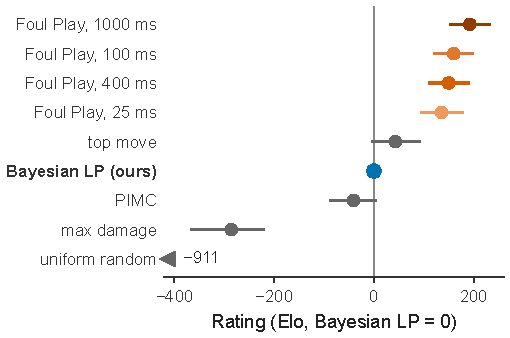
\includegraphics[width=\columnwidth]{figures/fig_gauntlet_col.pdf}
\caption{Real-Showdown round-robin tournament (1,800 games, 36 pairings): Bradley--Terry Elo with Bayesian LP fixed at 0 and 95\% bootstrap CIs. Foul Play's time is per sampled battle. Max damage plays the move with the highest base power $\times$ same-type bonus $\times$ type effectiveness. Uniform random ($-911$ [$-1495$, $-752$]) is off-scale.}
\label{fig:gauntlet}
\end{figure}

\begin{table}[t]
\centering\footnotesize\setlength{\tabcolsep}{2pt}
\caption{Real Showdown: score of the first-named bot [95\% CI] over seat-swapped pairs. Log loss in nats per scored turn. $^*$Pre-registered (prediction in parentheses).}
\label{tab:showdown}
\begin{tabular}{@{}>{\raggedright\arraybackslash}p{1.4in}lr@{}}
\toprule
Comparison & Result [95\% CI] & $n$ (pairs)\\
\midrule
\multicolumn{3}{@{}l}{\emph{Inside a turn: Bayesian LP~\cite{Yu26}}}\\
vs PIMC averaging & 0.559 [0.521, 0.597] & 298\\
\ \ same, in tournament & 0.538 [0.425, 0.650] & 40\\
vs Foul Play & 0.314 [0.279, 0.350] & 299\\
\ \ by search time & .317/.317/.275/.225 & 60 each\\
\multicolumn{3}{@{}l}{\emph{Across games: Hedge, style posterior~\cite{CBL06}}}\\
Hedge vs Foul Play & 0.311 [0.280, 0.341] & 399\\
Hedge vs Bayesian LP & 0.458 [0.421, 0.496] & 300\\
style posterior $-$ Hedge & $+0.024$ [$-0.018$, $+0.066$] & 397\\
\multicolumn{3}{@{}l}{\emph{Search root: bandit vs RM$^+$, $N=2000$~\cite{Lis13}}}\\
UCB1, visit shares & 0.050 [0.031, 0.069] & 299\\
Exp3, visit shares & 0.063 [0.043, 0.082] & 296\\
UCB1, most-visited & 0.593 [0.555, 0.632] & 300\\
Exp3, most-visited & 0.495 [0.455, 0.535] & 295\\
\multicolumn{3}{@{}l}{\emph{Detection delay $d$ vs prediction $\hat d$ (\cref{prop:T5})}}\\
median $d/\hat d$; $\rho^*$ & 1.06; 0.86 & 20 ($\lambda{=}1$)\\
$d$ ratio, pre-switch $\times2^*$ & 2.09 (1.5--2.7) & 20 ($\lambda{=}1$)\\
$d$, forgetting $\lambda=0.98^*$ & 37.5 (35) & 10\\
\multicolumn{3}{@{}l}{\emph{Per-world style likelihood; other tests}}\\
log-loss gain$^*$ & 0.297 / 0.311 (rep.) & 200 / 200\\
win rate$^*$ ($t_9$) & $+0.063$ [$-0.011$, 0.136] & 200\\
\ \ replication$^*$ & $+0.008$; LB $-0.045$ & 200\\
lookahead posterior$^*$ & 3 / 3,620 changed & 32 games\\
joint set$\times$style, offline & $+0.001\pm0.001$ & 18 games\\
\bottomrule
\end{tabular}
\end{table}

\paragraph{Bayesian LP vs PIMC averaging.} The Bayesian matrix game~\eqref{eq:af} avoids strategy fusion; PokaiTrainer reports no PIMC baseline. With sampled play, the Bayesian-LP agent beats PIMC averaging at equal compute, both in-engine (4 worlds, 340\,ms per move) and on real Showdown (\cref{tab:engine,tab:showdown}). The two settings use different belief models. With top-move play, neither the in-engine difference nor the tournament's is separable from zero. In-engine, the two agents pick different top moves on 14.9\% of logged decisions. These decisions carry a disproportionate share of PIMC averaging's loss: 32\% of the total, with a median of 1.33\% of the payoff range against 0.06\% elsewhere. So one game over the worlds is the better per-turn object for sampled play, but it does not close the gap to search.

\paragraph{Round-robin tournament.} \Cref{fig:gauntlet} shows nine bots. Foul Play at 25--1000\,ms per sampled battle rates 135 to 192, against 0 for Bayesian LP. Bayesian LP's score against Foul Play trends down with search time, from 0.317 [0.242, 0.392] at 25\,ms to 0.225 [0.158, 0.292] at 1000\,ms, with overlapping CIs (\cref{tab:showdown}: 25, 100, 400 and 1000\,ms). Over the same range, Foul Play's median MCTS iterations per search grow from 17,000 to 377,000. The agent rates below Foul Play even at its shortest search time. PokaiTrainer's premise therefore does not transfer to this setting.

\paragraph{Hedge on Showdown.} As an implementation check of \cref{fact:hedge}, on all 10 matches the per-turn regret on normalised stage payoffs stays below the anytime bound (median 0.0042 vs 0.0277 at $T=2{,}056$). Hedge scores like the Bayesian-LP agent alone and loses to it head to head (\cref{tab:showdown}). The guarantee concerns normalised stage payoffs on $\Abar$, not win probability. Over 17,271 decisions against Foul Play, Hedge's regret against its best fixed expert is $0.0044\pm0.0002$ per scored turn. In our estimated stage games, the opponent falls $0.021\pm0.001$ short of our equilibrium style. A literal equilibrium opponent shows the same gap, so the gap reflects model mismatch, not Foul Play's regret.

\paragraph{Bandit roots.} By \cref{prop:bandit}, visit shares need summed regret $o(N)$, which UCB1 does not guarantee here~\cite{Lis13}. Bandit roots that play their visit shares lose heavily to an RM$^+$ root (\cref{tab:showdown}). Their median duality gaps are 0.058 (both), against $2\cdot10^{-5}$ for RM$^+$. Offline on logged matrices, UCB1's gap is 0.12--0.125. Playing the most-visited action wins with UCB1 and ties with Exp3. At these iteration counts, the decision rule drives the outcome, not the feedback model, and deterministic play beats an opponent that does not adapt. A best response that knows the root's algorithm, but not its worlds or seed, gains clearly only against the visit-share root ($+0.035$ [0.014, 0.057]).

\paragraph{Case study.} At turn 18 of a logged 34-turn win against Foul Play, the experts disagreed. Top move and sampled play favoured a switch to Shiftry, pure maximin favoured Mystical Fire, and the $\varepsilon$-safe best response favoured our Shadow Ball. With carried Hedge weights 0.52, 0.24, 0.12 and 0.12, the mixture put 65\% on Shiftry and 8.5\% on Shadow Ball. We played Shiftry; the opponent played Shadow Ball.

\subsection{Bayesian opponent memory: prediction vs win rate}
\label{sec:exp-belief}
\paragraph{Bayes as Hedge.} As an implementation check of \cref{prop:B1}, the posterior's final regret is $1.609=\ln5$ on all eight fully logged matches. Its log loss is 1.56--1.81 nats per scored turn, against 3.23--3.32 for a one-hot predictor (24-pair pilots). Win rate did not change detectably relative to Hedge. A pre-registered test against single-style bots passed its regret-identity, identifiability and ordering predictions. It failed its final-style prediction and 2 of 6 identification-speed clauses~\cite{ext}.

\paragraph{Live test of the detection delay.} This pre-registered test checks \cref{prop:T5}. The opponent bot switches from the cautious (maximin) style to the uniform style (30 matches, 10 per arm). No pre-registered prediction was refuted. Each match's delay matches its own posterior's prediction: the median ratio is 1.06, inside the band [0.7, 1.4], and $\rho=0.86\ge0.5$. Doubling the pre-switch phase multiplies the delay by 2.09. Forgetting at $\lambda=0.98$ gives 37.5 updates against a predicted 35. Without forgetting~\cite{KZ93} or fixed share~\cite{HW98}, a posterior carried over many games detects a switch slowly.

\paragraph{Per-world style likelihood.} It lowers next-action log loss by 0.297 [0.281, 0.314] nats per scored turn, and by 0.311 [0.291, 0.331] in a pre-registered replication. Its win-rate gain did not replicate. On seeds 1--200 the gain was $+0.063$ (iid CI [0.003, 0.122]), but it was not robust to clustering by match ($t_9$ CI [$-0.011$, 0.136]). Seeds 201--400 gave $+0.008$ (LB $-0.045$). An offline analysis, not pre-registered, shows that restricting the likelihood to each world's legal actions accounts for the whole gain ($+0.324\pm0.031$ nats). A joint set$\times$style posterior adds $+0.001$. Updating the posterior inside the lookahead changed 3 of 3,620 actions and missed its pre-registered effect sizes. Better prediction shrinks only the belief term of \cref{thm:C}. Play does not improve, which is consistent with $\epsv$ dominating.

% =====================================================================
\section{Discussion and conclusion}
\label{sec:discussion}
\paragraph{Limitations.} Under load, the leaf evaluation occasionally searches deeper (1 in 17,000--19,000 calls). A deterministic control shows no detectable effect ($-0.008$ [$-0.057$, 0.040]). Unseeded sampling makes seed pairing weak (per-seed correlation 0.02--0.08). Earlier Showdown runs excluded 33 games lost to harness bugs, not at random~\cite{ext}.

\paragraph{Conclusion.} Our guarantees hold in the estimated matrix, whose leaf evaluation error does not shrink with compute (\cref{rem:leaf}) and plausibly dominates. Better beliefs do not move win rate. Next, we will train the evaluation function on exact terminal values.

\begingroup\small
\begin{thebibliography}{99}
\setlength{\itemsep}{1pt}\setlength{\parsep}{0pt}
\bibitem{FS99} Y.~Freund, R.~E.~Schapire. Adaptive game playing using multiplicative weights. \emph{Games and Economic Behavior} 29(1--2):79--103, 1999.
\bibitem{Zin07} M.~Zinkevich, M.~Johanson, M.~Bowling, C.~Piccione. Regret minimization in games with incomplete information. NeurIPS, pp.~1729--1736, 2007.
\bibitem{CBL06} N.~Cesa-Bianchi, G.~Lugosi. \emph{Prediction, Learning, and Games}. Cambridge University Press, 2006.
\bibitem{Yu26} M.~Yu. PokaiTrainer: Scaling equilibrium search to competitive Pok\'emon VGC. arXiv:2608.29197v2, 2026.
\bibitem{foulplay} P.~Mariglia. Foul Play: a competitive Pok\'emon Showdown battle bot. \url{https://github.com/pmariglia/foul-play}; engine \url{https://github.com/pmariglia/poke-engine}, 2024.
\bibitem{LW94} N.~Littlestone, M.~K.~Warmuth. The weighted majority algorithm. Information and Computation 108(2):212--261, 1994.
\bibitem{FS97} Y.~Freund, R.~E.~Schapire. A decision-theoretic generalization of on-line learning and an application to boosting. JCSS 55(1):119--139, 1997.
\bibitem{Tam14} O.~Tammelin. Solving large imperfect information games using CFR+. arXiv:1407.5042, 2014.
\bibitem{BMS19} N.~Burch, M.~Morav\v{c}\'{\i}k, M.~Schmid. Revisiting CFR+ and alternating updates. JAIR 64:429--443, 2019.
\bibitem{HW98} M.~Herbster, M.~K.~Warmuth. Tracking the best expert. Machine Learning 32(2):151--178, 1998.
\bibitem{ACF02} P.~Auer, N.~Cesa-Bianchi, P.~Fischer. Finite-time analysis of the multiarmed bandit problem. Machine Learning 47(2--3):235--256, 2002.
\bibitem{Lis13} V.~Lis\'y, V.~Kova\v{r}\'{\i}k, M.~Lanctot, B.~Bo\v{s}ansk\'y. Convergence of Monte Carlo tree search in simultaneous move games. NeurIPS, pp.~2112--2120, 2013.
\bibitem{Lon10} J.~Long, N.~R.~Sturtevant, M.~Buro, T.~Furtak. Understanding the success of perfect information Monte Carlo sampling in game tree search. AAAI, 2010.
\bibitem{AS18} S.~V.~Albrecht, P.~Stone. Autonomous agents modelling other agents: a comprehensive survey and open problems. \emph{Artificial Intelligence} 258:66--95, 2018.
\bibitem{KZ93} R.~Kulhav\'y, M.~B.~Zarrop. On a general concept of forgetting. \emph{Int.\ J.\ Control} 58(4):905--924, 1993.
\bibitem{GS15} S.~Ganzfried, T.~Sandholm. Safe opponent exploitation. \emph{ACM Trans.\ Economics and Computation} 3(2):8, 2015.
\bibitem{ext} Extended report. Supplementary material in the repository: \texttt{report/final.tex} and \texttt{report/current\_report.tex}.
\end{thebibliography}
\endgroup

\end{document}
